%%
%%
%%

\documentclass[cjk,dvipdfm,12pt]{beamer}
\usetheme{Hibi}
\usefonttheme{professionalfonts}
\usepackage{packages}

%%\mathversion{bold}

\AtBeginDvi{\special{pdf:tounicode EUC-UCS2}}

\title{Haskell$B$N(BArrow$B$N>R2p(B}
\subtitle{$B=i?4<T(BHaskell$BJY6/2q(B}
\author{$BF|HfLn(B $B7<(B}
\date{2011$BG/(B05$B7n(B25$BF|(B}

\begin{document}

\lstset{language=Haskell,basicstyle=\small\ttfamily}
  %% commentstyle=\textit,%
  %% classoffset=1,%
  %% keywordstyle=\bfseries,%
  %% frame=tRBl,framesep=5pt,%
  %% showstringspaces=false,%
  %% numbers=left,stepnumber=1,numberstyle=\footnotesize%


\frame{\titlepage{}}

\begin{frame}
\frametitle{$B:#2s$NN.$l(B}

\begin{itemize}
\item Arrow$B$C$F$I$s$J$b$N(B
\item Arrow$B$G$I$s$J$3$H$,$G$-$k$N$+(B
\item Arrow$B$r:n$k$K$O(B
\end{itemize}

\end{frame}

\begin{frame}
\frametitle{$B:#2s$NN.$l(B}

\begin{itemize}
\item {\color{red} Arrow$B$C$F$I$s$J$b$N(B}
\item Arrow$B$G$I$s$J$3$H$,$G$-$k$N$+(B
\item Arrow$B$r:n$k$K$O(B
\end{itemize}

\end{frame}

\begin{frame}
\frametitle{Arrow$B$C$F$I$s$J$b$N(B}

$BE,Ev$K@bL@$9$k$H(B \\
Arrow $B$H$OF~NO$,$"$C$F=PNO$,$"$k$b$N(B

\end{frame}

\begin{frame}[fragile]
\frametitle{Arrow$B$C$F$I$s$J7?(B}

$BNc$($P4X?t$O(B Arrow $B$G$9(B

\begin{lstlisting}
foo0 :: b -> c
foo1 :: (->) b c

-- (->) $B$O(B2$B0z?t$N(B Type Constructor
--  Either a b $B$H$+8+$?$3$H$"$j$^$9$h$M(B?

-- (->) $B$r(B Arrow a $B$G$"$k$h$&$J(B a $B$HCV$-49$($k$H(B
foo2 :: Arrow a => a b c
\end{lstlisting}
\end{frame}

\begin{frame}
\frametitle{$B:#2s$NN.$l(B}

\begin{itemize}
\item Arrow$B$C$F$I$s$J$b$N(B
\item {\color{red} Arrow$B$G$I$s$J$3$H$,$G$-$k$N$+(B}
\item Arrow$B$r:n$k$K$O(B
\end{itemize}

\end{frame}

\begin{frame}
\frametitle{Arrow$B$G$I$s$J$3$H$,$G$-$k$N$+(B}

$B%G!<%?%U%m!<$C$]$$$b$N$,=q$1$^$9(B\\
$BO@M}2sO)$H$+(B

\end{frame}

\begin{frame}[fragile]
\frametitle{$B=`Hw(B}

Arrow $B$G$"$k$h$&$J%*%V%8%'%/%H$,MQ0U$5$l$F$$$k$H$-$O(B arr $B$G4X?t$+$iJQ49$9$k$3$H$,$G$-$^$9(B

\begin{lstlisting}
arr :: Arrow a => (b -> c) -> a b c
\end{lstlisting}
\end{frame}

\begin{frame}[fragile]
\frametitle{$B2sO)$NNc(B - and}

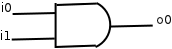
\includegraphics[height=1cm]{./And0.png}\\

\begin{itemize}
\item Arrow $B5-K!(B
\item $B$3$3$G(B Auto $B$O(B Arrow $B$K$J$C$F$$$^$9(B
\end{itemize}

\begin{lstlisting}
and2 :: (Bool, Bool) -> Bool
and2 = uncurry (&&)

and' :: Auto (Bool, Bool) Bool
and' = proc (i0, i1) -> do
         o0 <- arr and2 -< (i0, i1)
         id -< o0
\end{lstlisting}

\end{frame}

\begin{frame}[fragile]
\frametitle{$B2sO)$NNc(B - and}

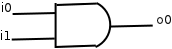
\includegraphics[height=1cm]{./And0.png}\\

\begin{itemize}
\item Arrow $B5-K!(B
\item $B$3$3$G(B Auto $B$O(B Arrow $B$K$J$C$F$$$^$9(B
\end{itemize}

\begin{lstlisting}
and2 :: (Bool, Bool) -> Bool
and2 = uncurry (&&)

and'' :: Auto (Bool, Bool) Bool
and'' = proc (i0, i1) -> do
         arr and2 -< (i0, i1)
\end{lstlisting}

\end{frame}

\begin{frame}[fragile]
\frametitle{$B2sO)$NNc(B - and}

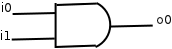
\includegraphics[height=1cm]{./And0.png}\\

\begin{itemize}
\item Arrow $B5-K!(B
\item $B$3$3$G(B Auto $B$O(B Arrow $B$K$J$C$F$$$^$9(B
\end{itemize}

\begin{lstlisting}
and2 :: (Bool, Bool) -> Bool
and2 = uncurry (&&)

and''' :: Auto (Bool, Bool) Bool
and''' =  arr and2
\end{lstlisting}

\end{frame}

\begin{frame}[fragile]
\frametitle{$B2sO)$NNc(B - half adder}

\begin{lstlisting}
xor :: Auto (Bool, Bool) Bool
xor =  proc i -> do
         m0 <- nand -< i 
         m1 <- or'  -< i
         and' -< (m0, m1)

hAdder :: Auto (Bool, Bool) (Bool, Bool)
hAdder =  
  proc i -> do
    o0 <- xor  -< i
    o1 <- and' -< i
    id -< (o1, o0)
\end{lstlisting}
\end{frame}

\begin{frame}

\begin{itemize}
\item Arrow$B$C$F$I$s$J$b$N(B
\item Arrow$B$G$I$s$J$3$H$,$G$-$k$N$+(B
\item {\color{red} Arrow$B$r:n$k$K$O(B}
\end{itemize}

\end{frame}

\begin{frame}
\end{frame}

\end {document}
